This panel is where the user selects the outputs to be displayed when
the simulation runs. There are two options available in the pull-down
menu:
\begin{enumerate}
\item Standard Earthquake (\ref{subsec:sectionStandardEarthquake})
\item User Defined (\ref{subsec:sectionUserDefined})
\end{enumerate}





\subsection{Standard Earthquake}\label{subsec:sectionStandardEarthquake}
When the user selects standard Earthquake there are no additional
inputs required. The standard earthquake EDP generator will ensure the
the max absolute value of the following are obtained:
\begin{enumerate}
\item Relative Floor displacements:
\item Absolute Floor Accelerations
\item Interstory Drifts
\end{enumerate}

The results will contain results for these in abbreviated form:
\begin{itemize}
\item PFD peak relative floor displacement $1-PFD-FLOOR_CLINE$
\item PFA peak floor acceleration (relative + ground motion):
  $1-PFA-FLOOR-CLINE$
\item PID peak inter-story drift: $1-PID-STORY-CLINE$
\end{itemize}

\subsection{User Defined}\label{subsec:sectionUserDefined}
This panel shown in \Cref{fig:userEDP} allows the user to provde to determine their own output and process it. When using this option the user provides additional data:

\begin{figure}[!htbp]
  \centering {
    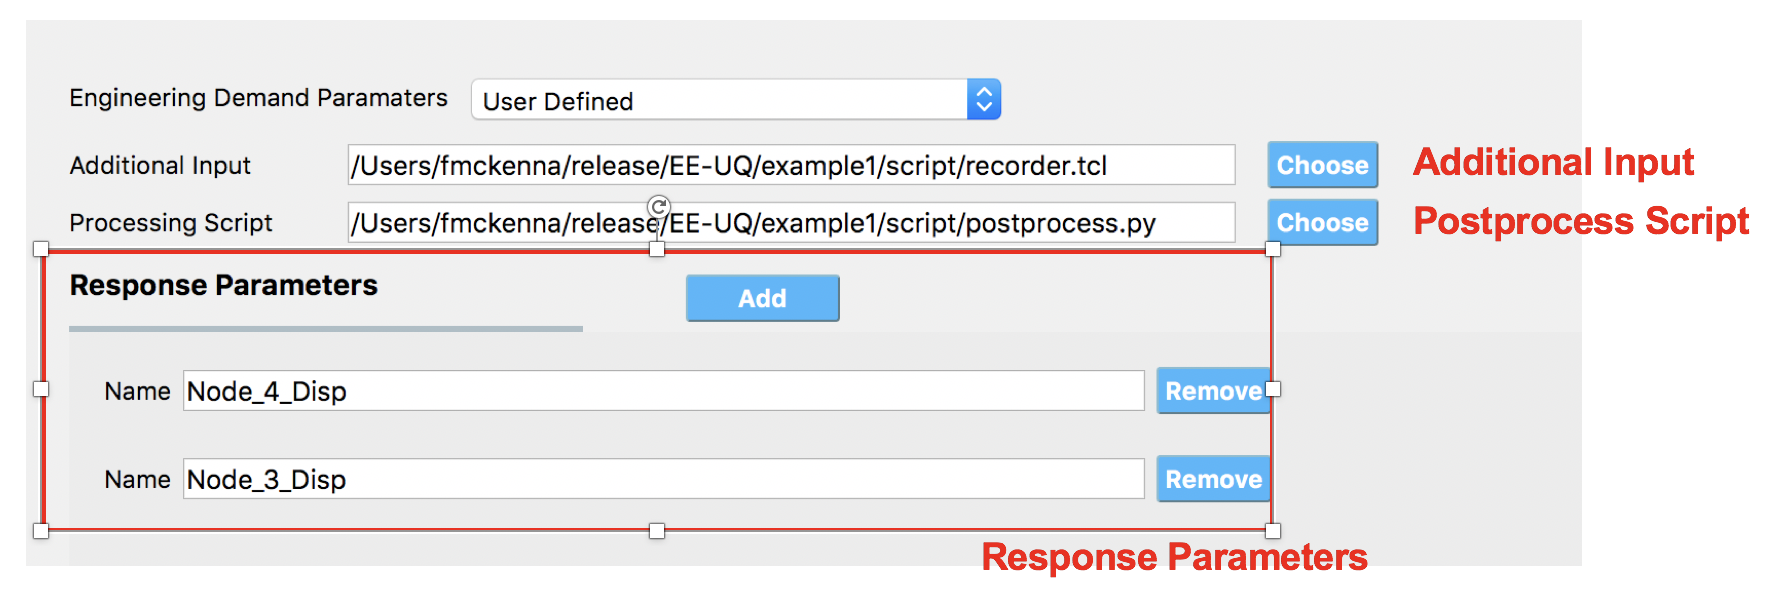
\includegraphics[width=0.8\textwidth]
    {usage/figures/userDefinedEDP.png} }
  \caption{userEDP}
  \label{fig:userEDP}
\end{figure}

\begin{enumerate}
\item Additional Input: These are additional commands that are invoked
  by the analysis application before the transient analysis is
  performed. For example, foe OpenSees this would be a script
  containing a series of recorder commands. \\

For example, a recorder file passed to OpenSees might look like the following:
\begin{verbatim}
recorder EnvelopeNode -file node.out -node 1 2 3 4 -dof 1 disp
recorder EnvelopeElement -file ele.out -ele 1 2 3 forces
\end{verbatim}

\item Postprocess Script: This is a python script that will be invoked
  after the finite element application has run. It must be provided by
  the user. It's purpose is to process the output files and create a
  single file, results.out. This file must contain a single line with
  as many entries as EDP's specified.

For example, a postprocessing file that would take the outputs from the analysis to create the results file might look like the following:

\begin{python}
#!/usr/bin/python                                                                 

import sys
import re

EDPs = ['Node_4_Disp', 'Node_3_Disp']

inputArgs = sys.argv

with open ('node.out', 'rt') as inFile:
    line = inFile.readline()
    line = inFile.readline()
    line = inFile.readline()
    displ = line.split()
    numNode = len(displ)

inFile.close

#                                                                                 
# now process the input args and write the results file                           
#                                                                                 

outFile = open('results.out','w')

#                                                                                 
# note for now assuming no ERROR in user data                                     
#                                                                                 

for i in EDPs[0:]:
    print i
    theList=i.split('_')

    if (theList[0] == 'Node'):
        nodeTag = int(theList[1])

        if (nodeTag > 0 and nodeTag <= numNode):
            if (theList[2] == 'Disp'):
                nodeDisp = displ[nodeTag-1]
                outFile.write(nodeDisp)
                outFile.write(' ')
            else:
                outFile.write('0. ')
        else:
            outFile.write('0. ')
    else:
        outFile.write('0. ')

outFile.close
\end{python}



\item Response Parameters. This is an area in which the user
  associates a variable name with the column of the results output
  file. If the process script has an array of strings named named
  EDP's the script, the Response Parameters will be initially set with
  these values from the script.
\end{enumerate}

